\section{Data}\label{sec:data}

\subsection{Photometric data}

Описание данных SDSS, PanStarrs, DESI LIS. Какие фильтры используем, какие признаки вычисляем. Указать формулы, которые используем для подсчета величин.

Таблица с глубиной измерений (см Brescia table 1)

Графики с покрытием неба? Чтобы понимать, какую модель где можно использовать.

\achtung{У Brescia была большая таблица с чуввствительностями. Доразобраться, как онаа строится?}

\subsection{Spectral data}

\begin{figure*}
    \centering
    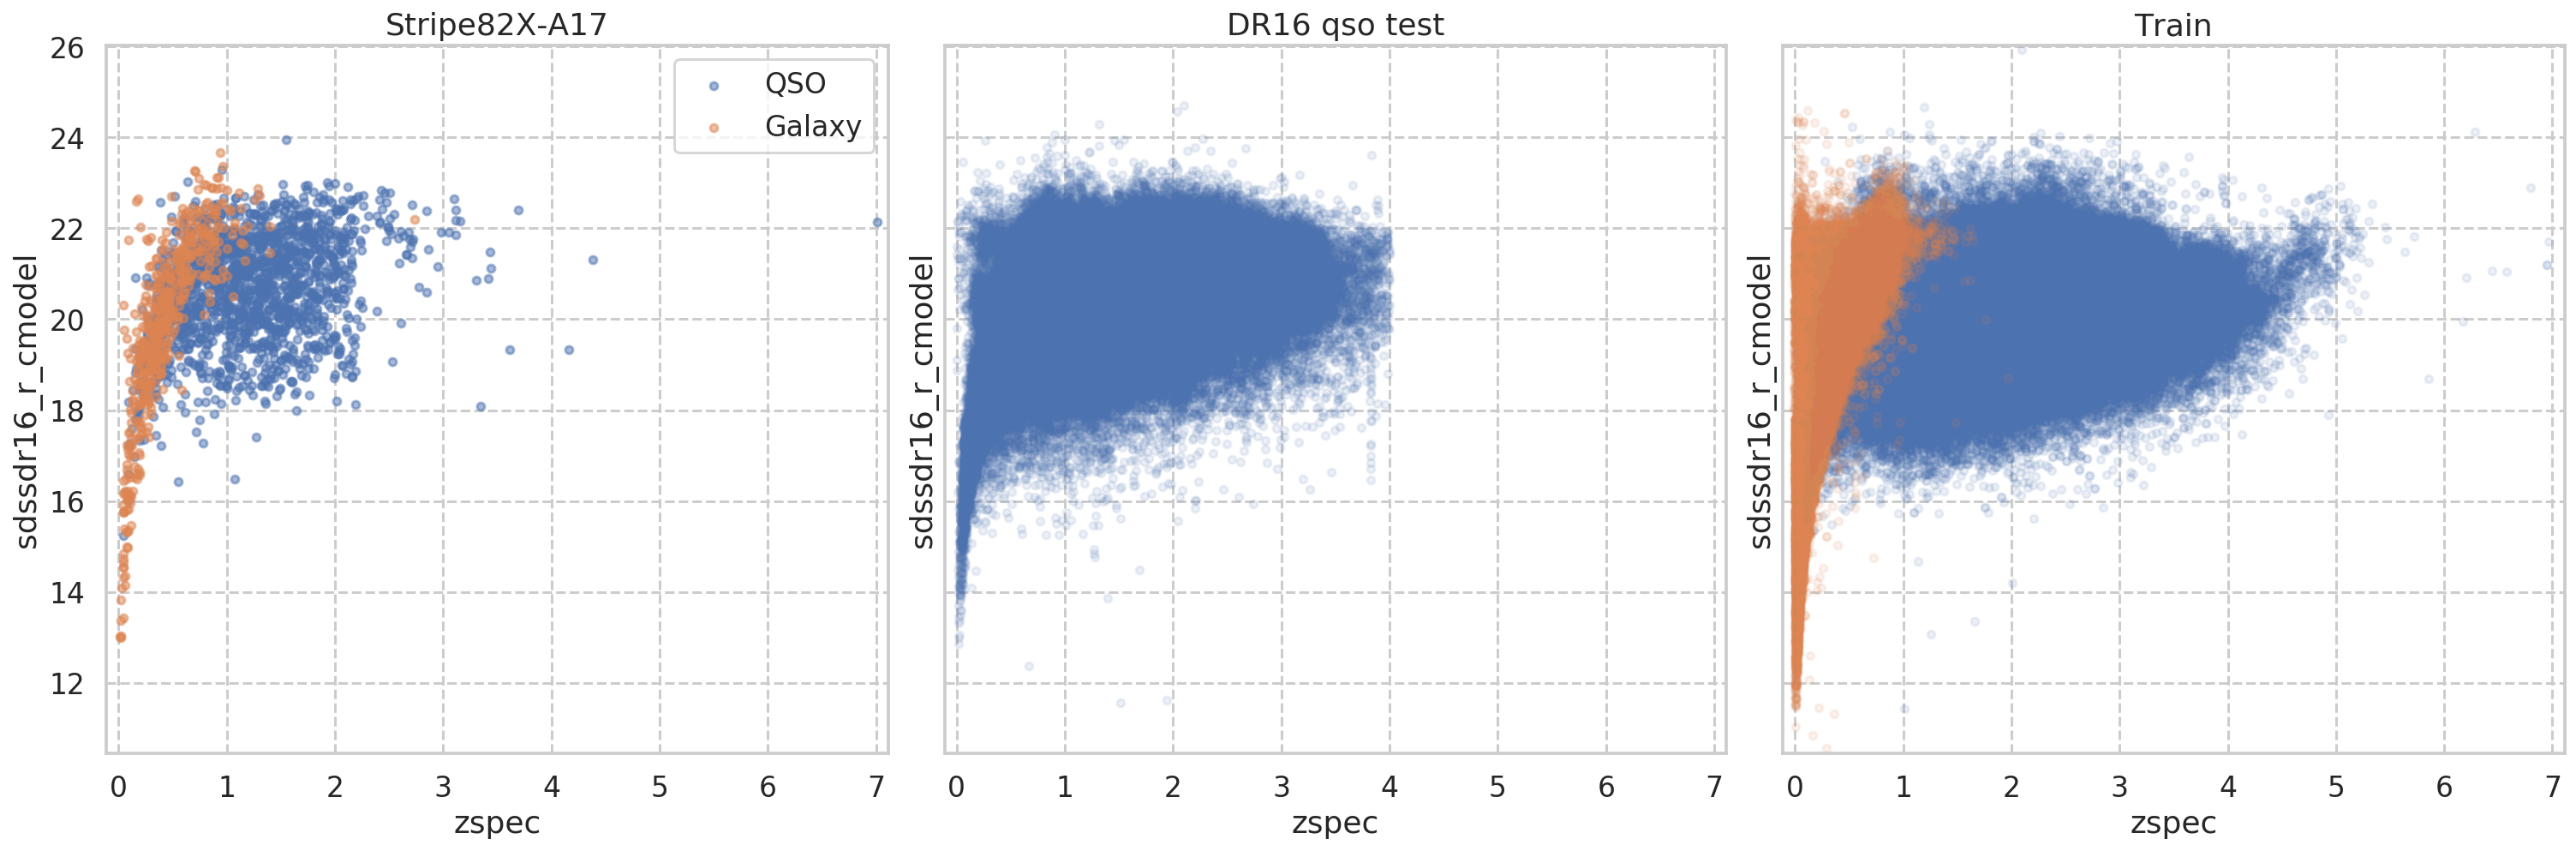
\includegraphics[width=\linewidth]{images/spectroscopic-coverage.png}
    \caption{Spectroscopic coverage of samples}
    \label{fig:spectroscopic_coverage}
\end{figure*}

\subsubsection{SDSS}

Описание числа объектов спектраальной выборки SDSS.

Сказать про DR14q Paris, и как отбираются надежные объекты DR16. Привести картинку из презенташки.

\subsubsection{Stripe82X}

Не уверен, где лучше описать выборку - тут или в \ref{sebsebsec:test}?

Вкратце описать выборку, что она из себя представляет, что это наилучший тест для рентгеновских квазаров, сослаться на работу Ananna.

\subsection{Datasets}

\subsubsection{Train}

Как составлены обучающие выборки (рентгеновская, оптическая).

Привести скаттерплоты zspec(mag\_r), как в Brescia, чтобы показать спектроскопическое покрытие ("spectroscopic coverage"), сравнить его со Stripe82X

\subsubsection{Test}\label{sebsebsec:test}

Описание выборки 200 тыс. квазаров, как составлена. Что мы её используем, чтобы, в первую очередь, адекватно протестироваться на далеких объектах.

+ В качестве теста используем Stripe82X.

+ для обеих выборок привести спектроскопическое покрытие.